\documentclass[12pt,a4paper]{report}

\usepackage[pdftex]{graphicx}
\graphicspath{ {img/} }


\usepackage{titlesec}
\usepackage[english]{babel}
\usepackage{enumitem}          
\usepackage[nottoc]{tocbibind}
\usepackage[T1]{fontenc}
\usepackage[utf8]{inputenc}
\usepackage{lmodern}
\usepackage[autostyle]{csquotes}
\usepackage[hyperref=true,
	    backend=bibtex,
            url=false,
            isbn=false,
            backref=true,
            style=numeric,
            maxcitenames=3,
            maxbibnames=100,
            block=none]{biblatex}
% always load after biblatex
\usepackage[colorlinks=true,linkcolor=blue,urlcolor=black,bookmarksopen=true]{hyperref}
\bibliography{references}

\titleformat{\chapter}
  {\Large\bfseries} % format
  {}                % label
  {0pt}             % sep
  {\huge}           % before-code

\title{OCR using Neural Network}

\begin{document}
\renewcommand\bibname{References}


\begin{titlepage}
	\centering
	
\includegraphics[width=40mm]{img/tu}\par\vspace{1cm}
	{\scshape\LARGE Tribhuwan University \par}

	\textsc{\bfseries INSTITUTE OF ENGINEERING}\\
	\textsc{\bfseries PULCHOWK CAMPUS}\\

	\vspace{1cm}
	{\huge\bfseries Optical Character Recognition using Neural Network\par}
	{\scshape In Fulfillment of Software Engineering Project\par}
	\vspace{1.5cm}
\normalsize Submitted by \\
\begin{table}[h]
\centering
\begin{tabular}{lr}\hline \\
		Dinesh Bhattarai    &   072 BCT 512\\
		Aashutosh Poudel    &   072 BCT 502\\
		Jeevan Thapa        &   072 BCT 514\\
		Rupesh Shrestha     &   072 BCT 530\\
		Simon Dahal         &   072 BCT 538\\
		Yogesh Rai          &   072 BCT 548\\ \hline
\end{tabular}
\end{table}
	\vspace{1.1cm}
	\textsc{\bfseries Submitted To}
	\
	
	{\scshape DEPARTMENT OF ELECTRONICS AND COMPUTER ENGINEERING\par}
\

	{\large \today\par}
\end{titlepage}

%\begin{titlepage}

\begin{center}

\textup{\small {\bf Project} \\ Report}\\[0.2in]

% Title
\Large \textbf {Optical Character Recognition using Neural Network}\\[0.5in]

       \small \emph{Submitted in partial fulfillment of\\
        the requirements for}
        \vspace{.2in}

       {\bf Software Engineering \\in\\ Computer Science and Engineering}\\[0.5in]

% Submitted by
\normalsize Submitted by \\
\begin{table}[h]
\centering
\begin{tabular}{lr}\hline \\
		Dinesh Bhattarai    &   072 BCT 512\\
		Aashutosh Poudel    &   072 BCT 502\\
		Jeevan Thapa        &   072 BCT 514\\
		Rupesh Shrestha     &   072 BCT 530\\
		Simon Dahal         &   072 BCT 538\\
		Yogesh Rai          &   072 BCT 548\\ \hline
\end{tabular}
\end{table}

\vspace{.1in}
Under the guidance of\\
{\textbf{Bishwash Pokhrel}}\\[0.2in]

\vfill

% Bottom of the page

\includegraphics[width=0.18\textwidth]{./tu}\\[0.1in]
\Large{Department of Electronics and Computer Engineering}\\
\normalsize
\textsc{IOE, Pulchowk Campus}\\
Pulchowk, Patan, Nepal\\
\vspace{0.2cm}

\end{center}
\end{titlepage}


\pagenumbering{roman}
%\newpage
\thispagestyle{empty}

\begin{center}

\huge{Department of Computer Science and Engineering}\\[0.5cm]
\normalsize
\textsc{National Institute of Technology Calicut}\\[2.0cm]

\emph{\LARGE Certificate}\\[2.5cm]
\end{center}
\normalsize This is to certify that this is a bonafide record of the project presented by the students whose names are given below during <Monsoon/Winter and Year here> in partial fulfilment of the requirements of the degree of Bachelor of Technology in Computer Science and Engineering.\\[1.0cm]

\begin{table}[h]
\centering
\begin{tabular}{lr}
Roll No & Names of Students \\ \\ \hline
\\
<Roll no here> & <Name here> \\ 
<Roll no here> & <Name here> \\
<Roll no here> & <Name here> \\
\end{tabular}
\end{table}

\vfill


% Bottom of the page
\begin{flushright}
<Guide name here>\\
(Project Guide)\\[1.5cm]
<Coordinator name here>\\
(Course Coordinator)\\
\end{flushright}

\begin{flushleft}
Date:
\end{flushleft}

\cleardoublepage
\addcontentsline{toc}{chapter}{Acknowledgements}
\chapter*{Acknowledgments}
We would like to express our sincere gratitude to our teachers Mr. Biswas Pokhrel and Mrs. Rama Bastola for providing their invaluable guidance, comments and suggestions throughout the course of the project. We would also like to thank the Department of Electronics and Computer Engineering for providing us this golden opportunity to apply the theoretical concepts we have learned during the course that ultimately helped us in understanding the practical side of it.

We would also like to thank our friends and seniors who helped us in choosing the right tools, algorithms and techniques for the project. Also, we must acknowledge our deep sense of gratitude to the mentors of DN: AI Developers Nepal group and their AI Saturdays Meet Up which helped us to get started with our project and gain knowledge of various topics in AI. 
\newpage

\addcontentsline{toc}{chapter}{Abstract}
\chapter*{Abstract}

Optical Character Recognition systems solve the problem of digitizing handwritten or typed documents, forms, letters, etc. OCR systems are widely used to automate and speed up data entry process thereby reducing human errors. The OCR system developed by us has a web interface that is capable of taking input through a camera and giving the output of the recognized text to the user. A system capable of recognizing both handwritten and written English alphabets has been developed as part of this project. 

A four layer CNN architecture has been trained and used in order to classify the individual alphabets in the input. Further pre-processing and feature extraction of the input images is done using algorithms like MSER, Gaussian filters, etc. The input image is taken through the camera or through file upload to the system. The feature extraction part is then done to collect inputs for the trained model. The output given by the model is the recognized character output of the entire system.
An overall accuracy of 83\% has been observed with the system. Further improvements in the system can be made using a more robust set of features and a much larger dataset to improve the accuracy.

\textbf{Keywords: OCR, handwriting recognition, CNN, neural networks, digits recognition, MSER, Canny Edge Detection}

\tableofcontents
\listoffigures

\newpage
\pagenumbering{arabic}

\chapter{Introduction}

\section{Background and Recent Research}
\subsection{<any sub section here>}

\subsection{Literature Survey}

\subsubsection{<Sub-subsection title>}
some text\cite{citation-1-name-here}, some more text

\subsubsection{<Sub-subsection title>}
even more text\footnote{<footnote here>}, and even more.

\section{Motivation}

\chapter{Methodology}

\section{Use case diagram}

\begin{figure}[htb]
\centering
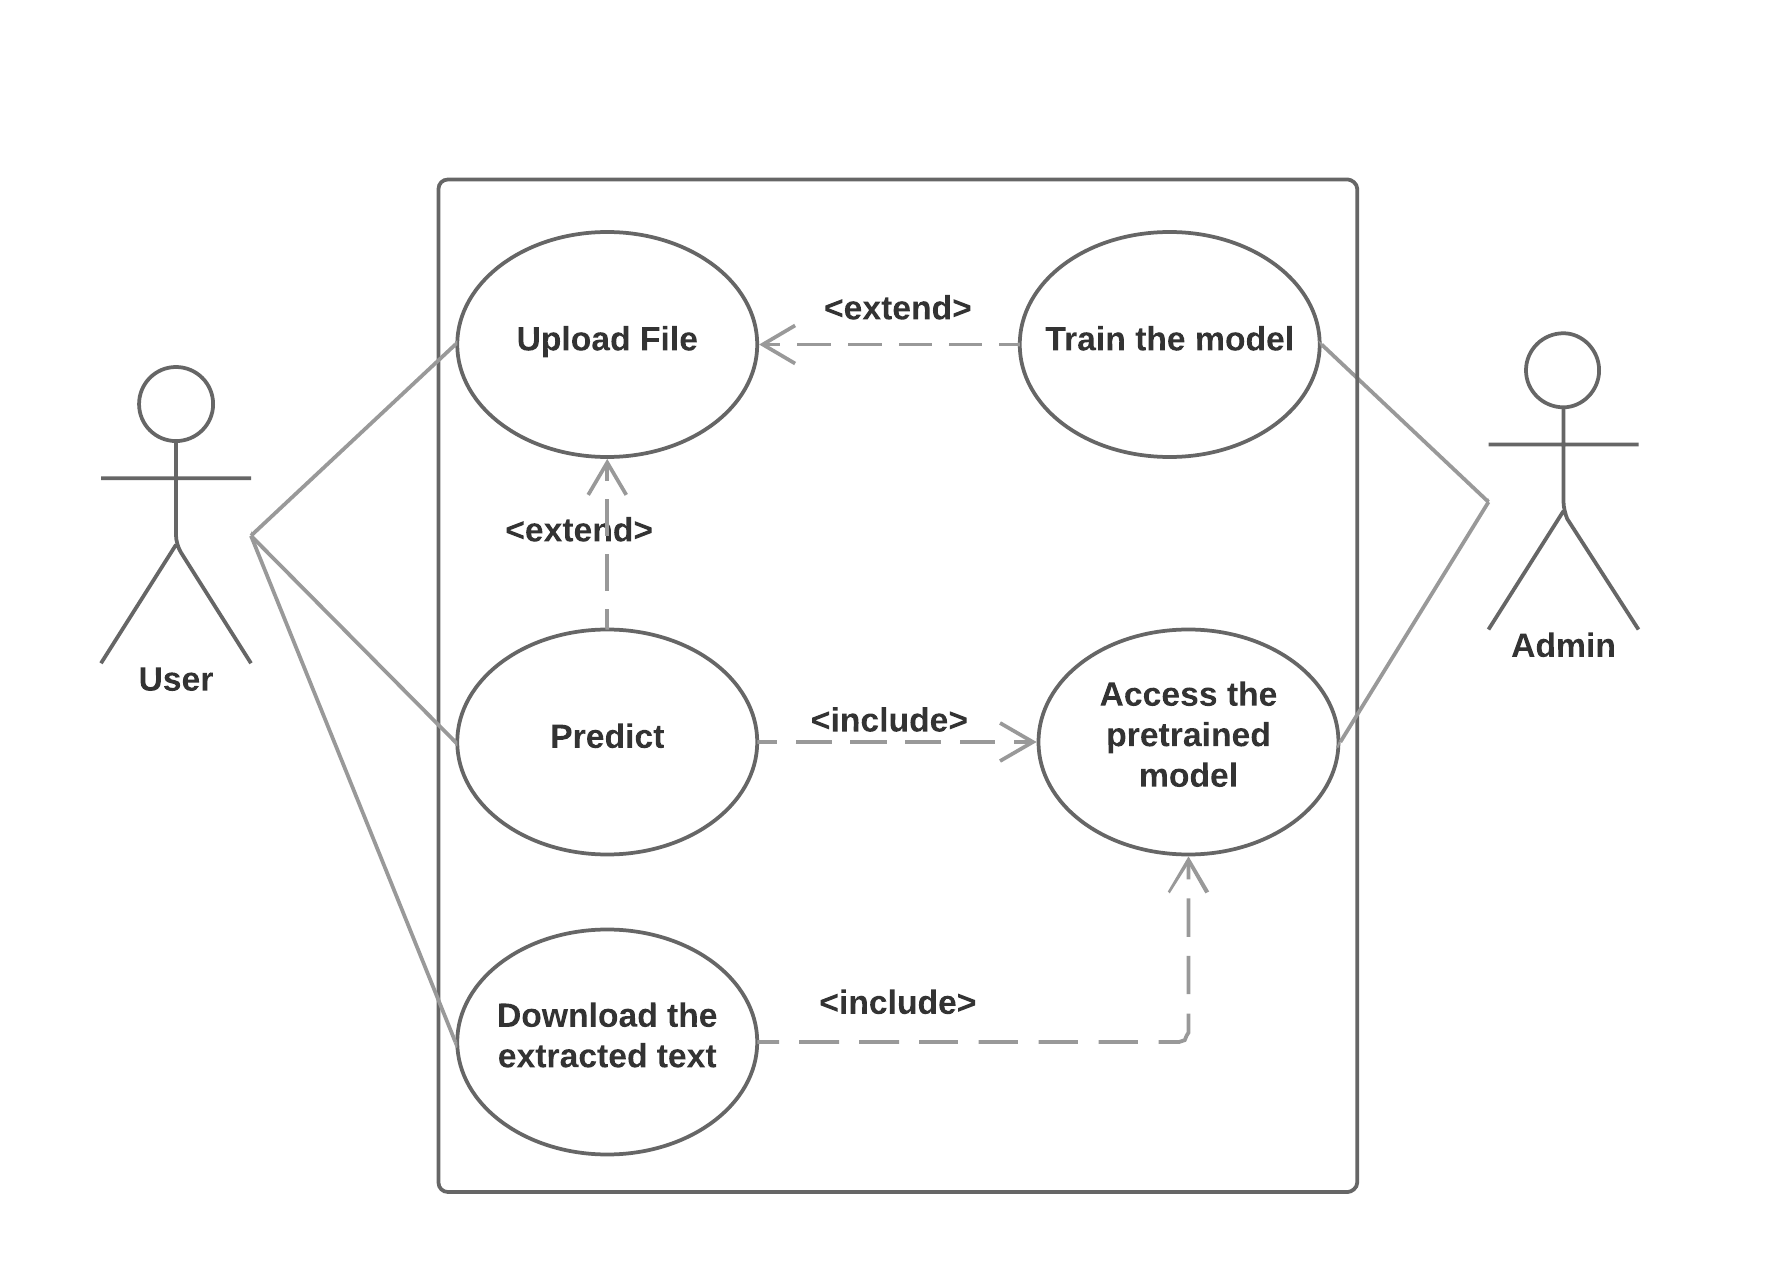
\includegraphics[scale=1]{UseCase}
\caption{Use Case diagram}
\end{figure}

The purpose of a use case diagram here is to demonstrate the different ways that a user might interact with a system. The main actors in our systems are the actual users who use it and the administrator responsible for updating or training the model used in the system. The user uses the system in order to predict the text present in the image by uploading the image and gets the output from the prediction model as indicated in the relationship above.

Also, after the user chooses to predict the text in the image, the pre-trained model is automatically accessed to produce the required output as shown by the relationship between the two use cases.

\section{Level 0 Data Flow Diagram}

\begin{figure}[htb]
\centering
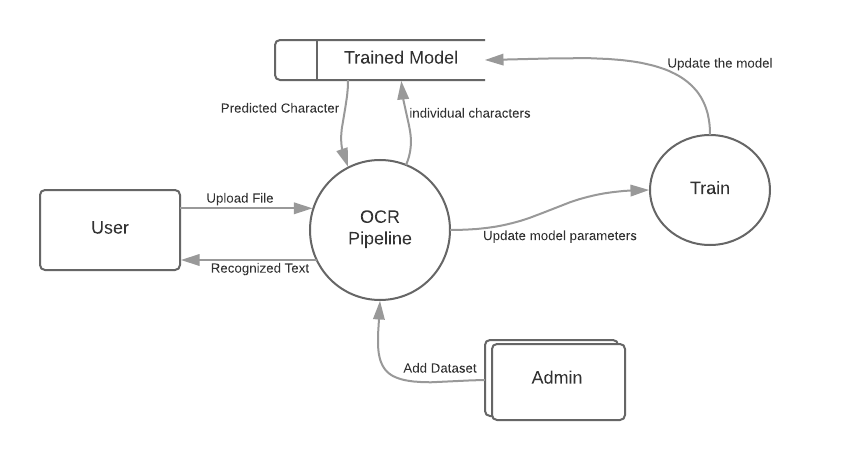
\includegraphics[scale=1]{level0}
\caption{Level 0 Data Flow Diagram}
\end{figure}

DFD Level 0, also called Context Diagram, shows a basic overview of the whole system. The above diagram provides an at-a-glance view, showing the system as a single high-level process, with its relationship to external entities. The circles in the diagram represent a process, the rectangular boxes represent entities and the arrows indicate the data flow direction.

In our system, the external entities are the user and the admin. The OCR pipeline and the trained model are internal to the system. The user directly interacts with the pipeline giving image file as an input and gets the desired output in the form of text from the pipeline. Similarly the admin also interacts with the pipeline with the help of dataset that is used for training as well as testing purposes. Further, the pipeline interacts with the trained prediction model to generate the approximate match of the input character. It can also train the model using the dataset provided by the administrator.

\section{Level 1 Data Flow Diagram}

\begin{figure}[htb]
\centering
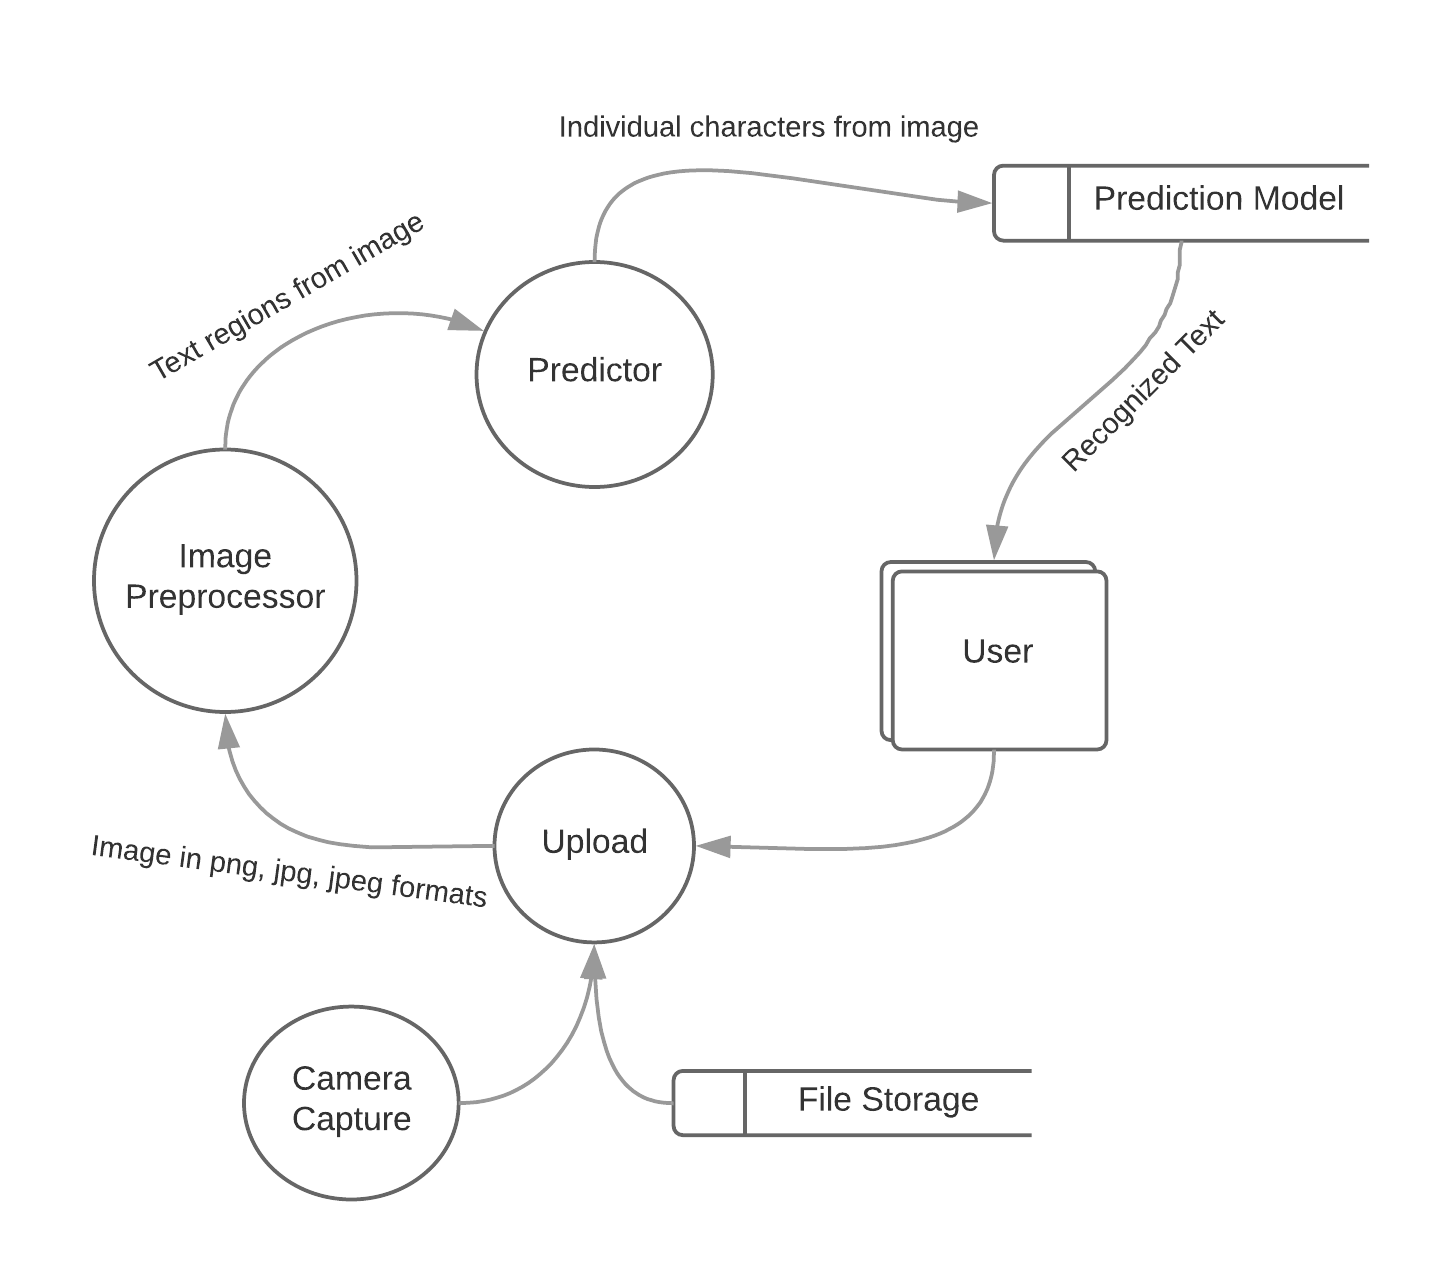
\includegraphics[scale=1]{level1}
\caption{Level 1 Data Flow Diagram}
\end{figure}


DFD Level 1 provides a more detailed breakout of pieces of the Context Level Diagram. The above level 1 DFD diagram of our system shows the OCR pipeline in more detail.

It includes an input mechanism through an external device like camera or through a file storage unit. The OCR pipeline consists of an image processor unit which applies various image processing algorithms to the image to identify text regions in the image. The next processes consists of predicting the text regions with the individual characters separated from the image and updating the user of the identified texts present in the image. 



\section{Level 2 Data Flow Diagram}

DFD Level 2 goes one step deeper into parts of Level 1. 

\begin{figure}[htb]
\centering
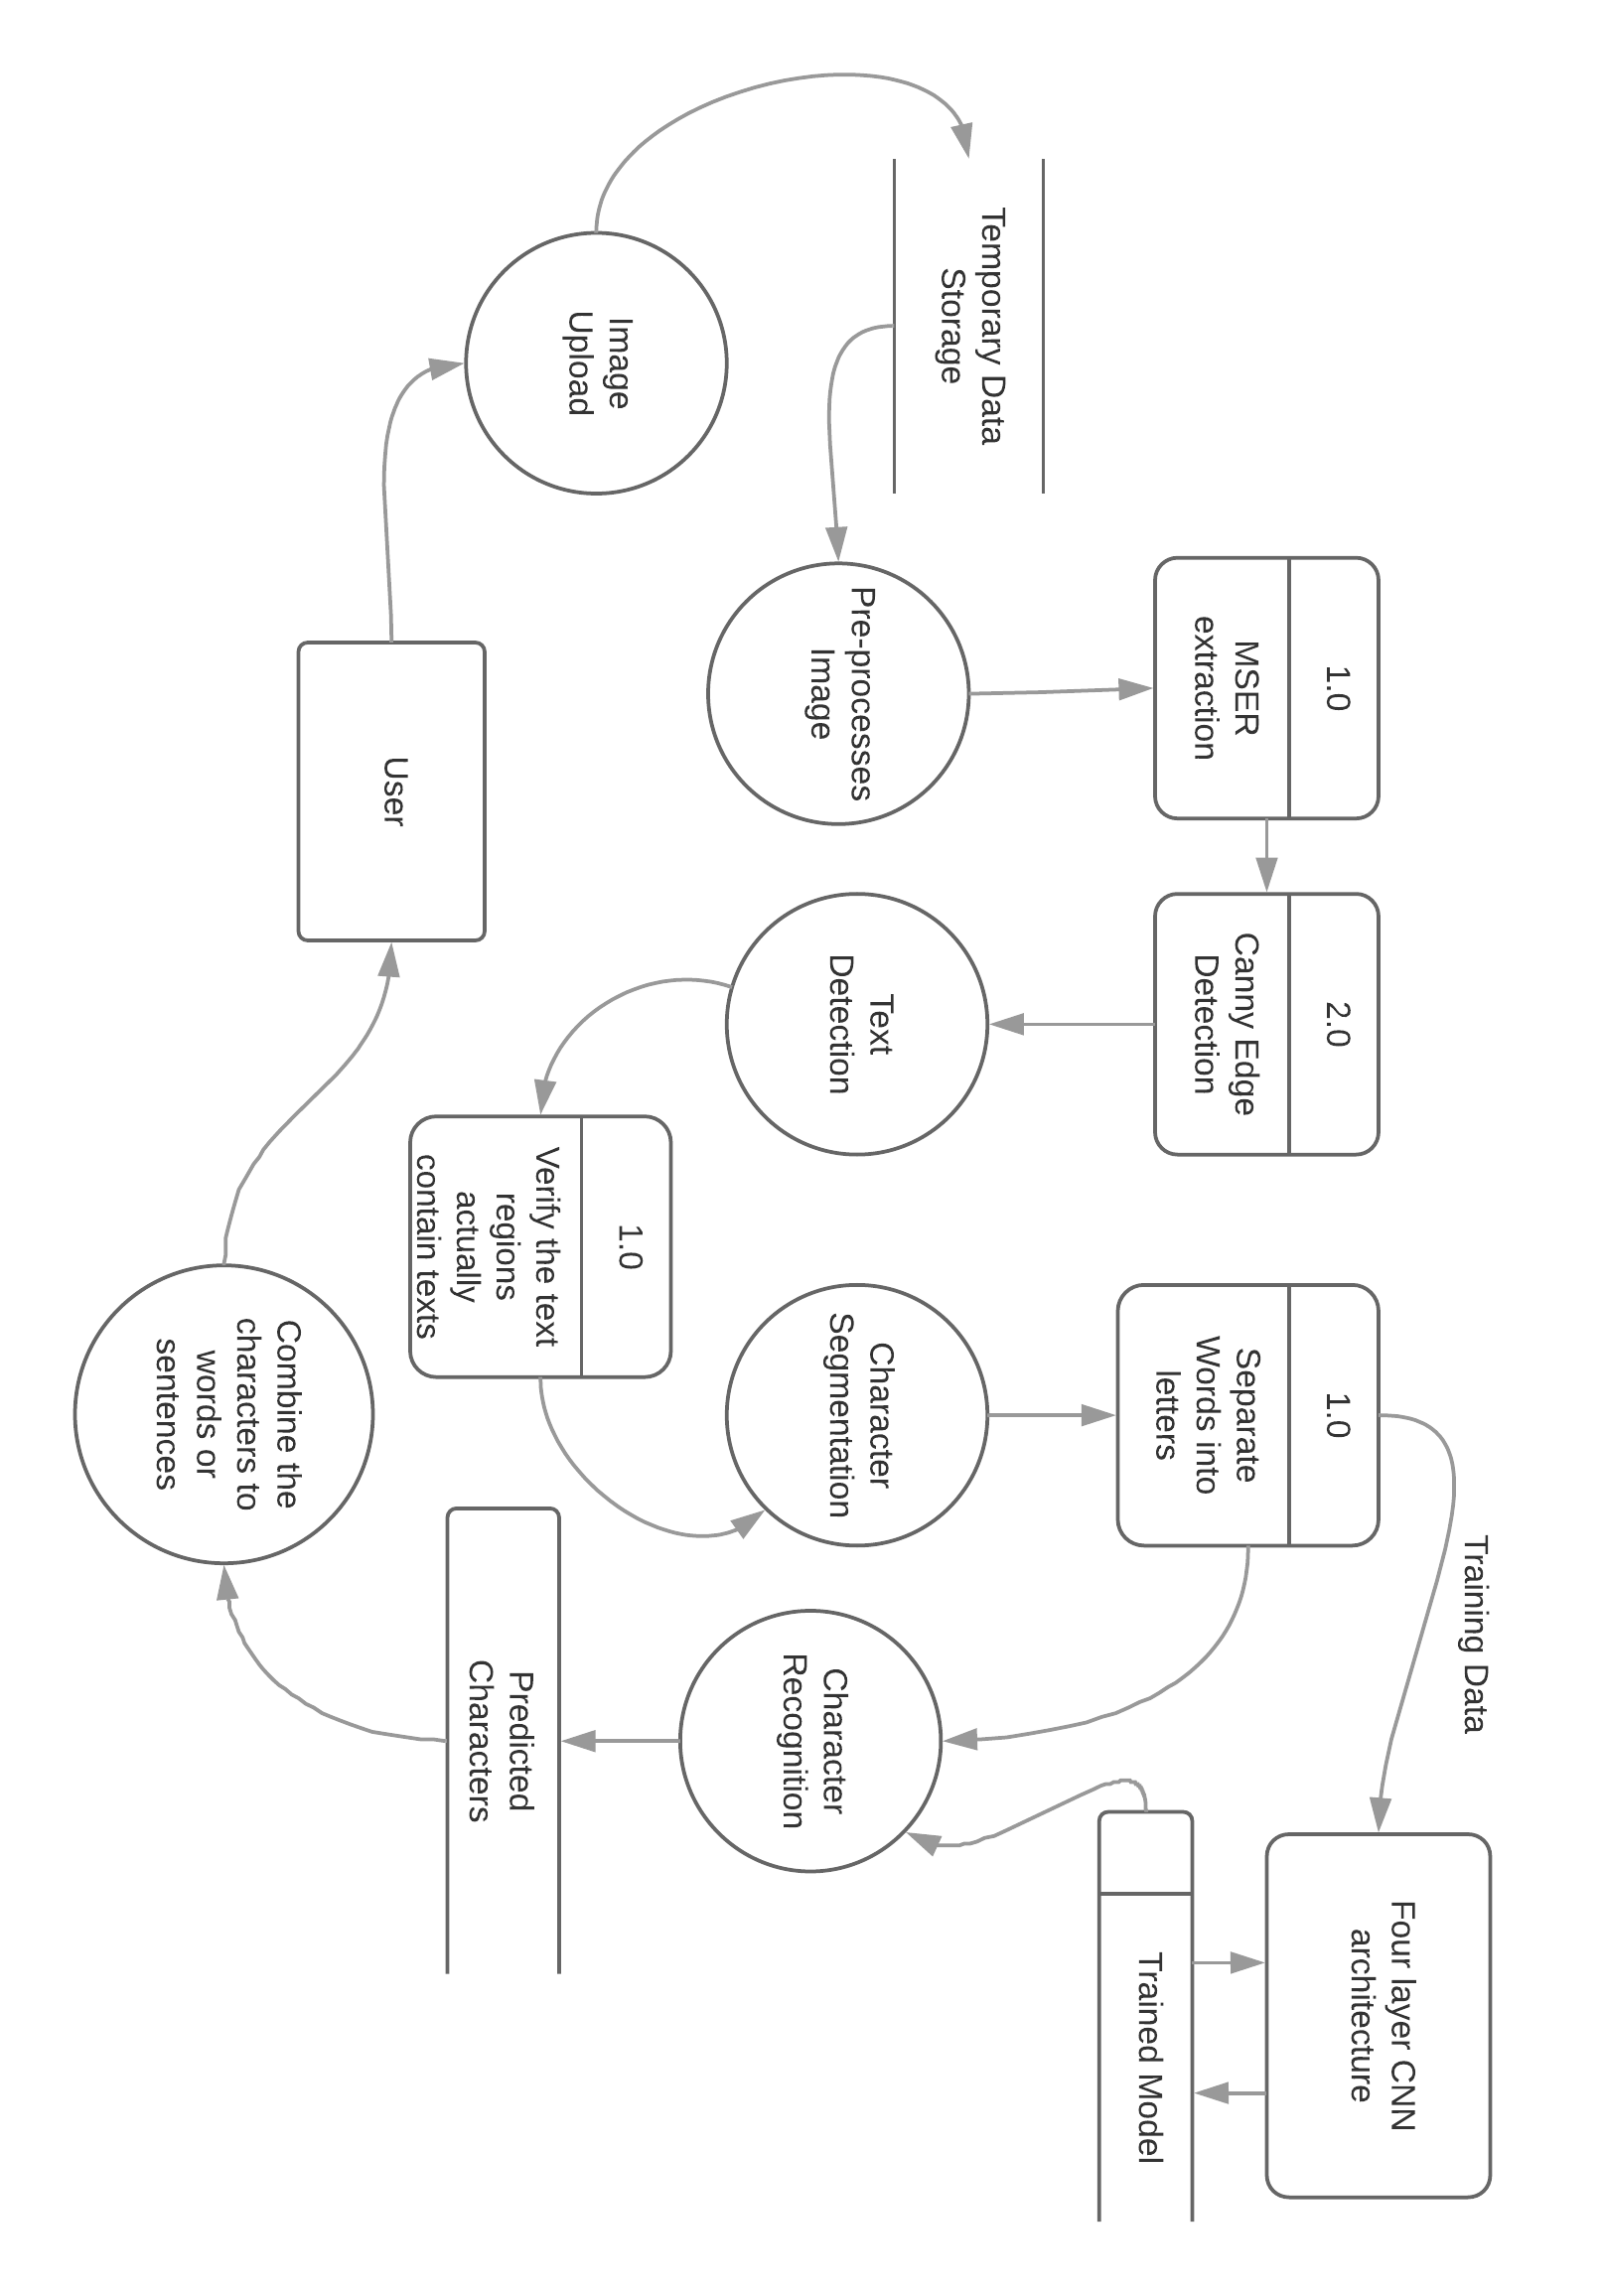
\includegraphics[scale=1]{level2}
\caption{Level 2 Data Flow Diagram}
\end{figure}

Thus the OCR pipeline from Level 1 is further divided into its constituent’s parts. The user interacts with the system using a web interface to upload the image file as well as get the output of the system. The image is then pre-processed using binarization, extraction using a combination of MSER and Canny Edge detection. After the text regions are obtained the regions gets segmented into characters and fed into the recognition engine. The recognition engine uses a pre-trained model trained by a four layer CNN architecture to predict the approximate output of the character or text. The predicted characters are combined to form words or sentences that is displayed to the user.

\section{Entity Relationship Diagram}

\begin{figure}[htb]
\centering
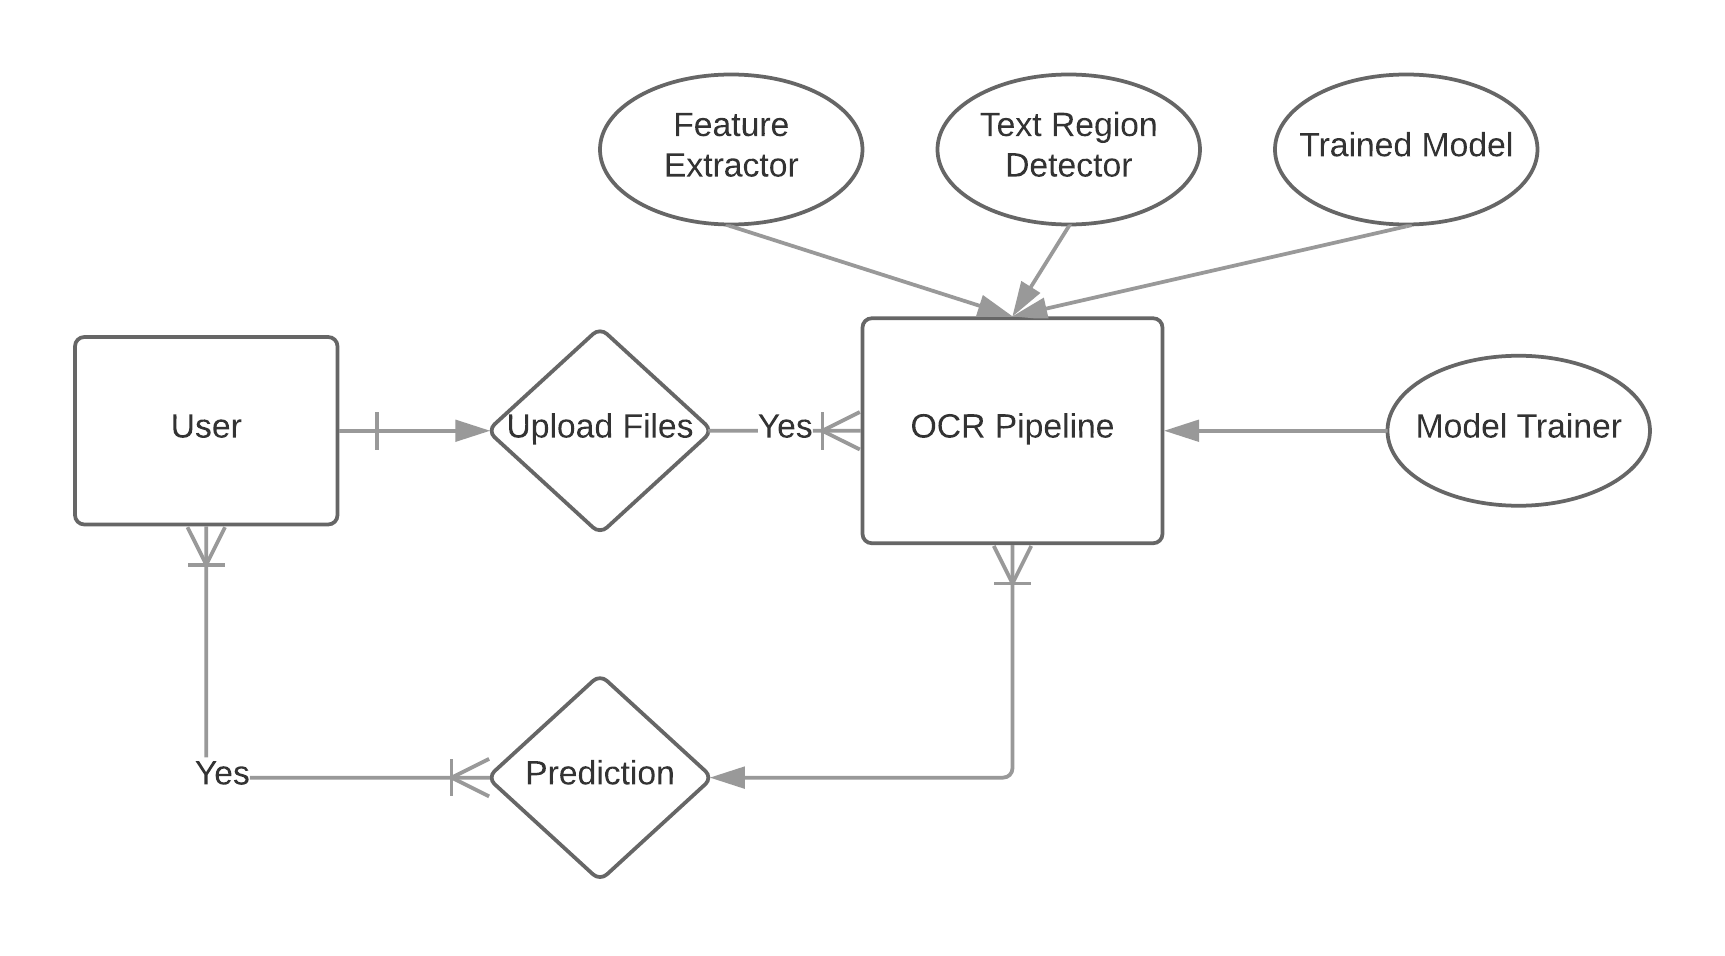
\includegraphics[scale=0.7]{ERD}
\caption{Entity Relationship Diagram}
\end{figure}


An Entity Relationship (ER) diagram shows how entities like people, objects, or concepts relate to each other within a system. In an ER diagram, the rectangular boxes represent the objects, or entities, diamonds represent the relationship between the entities, and an oval represents an attribute of an entity.

In the proposed system we have two major entities the user and the OCR pipeline. A user can upload one or many files at a time to the system. The pipeline has various components that analyses the given image and prints the gives the output of the images to on or many users. 

\section{Activity Diagram}

\begin{figure}[htb]
\centering
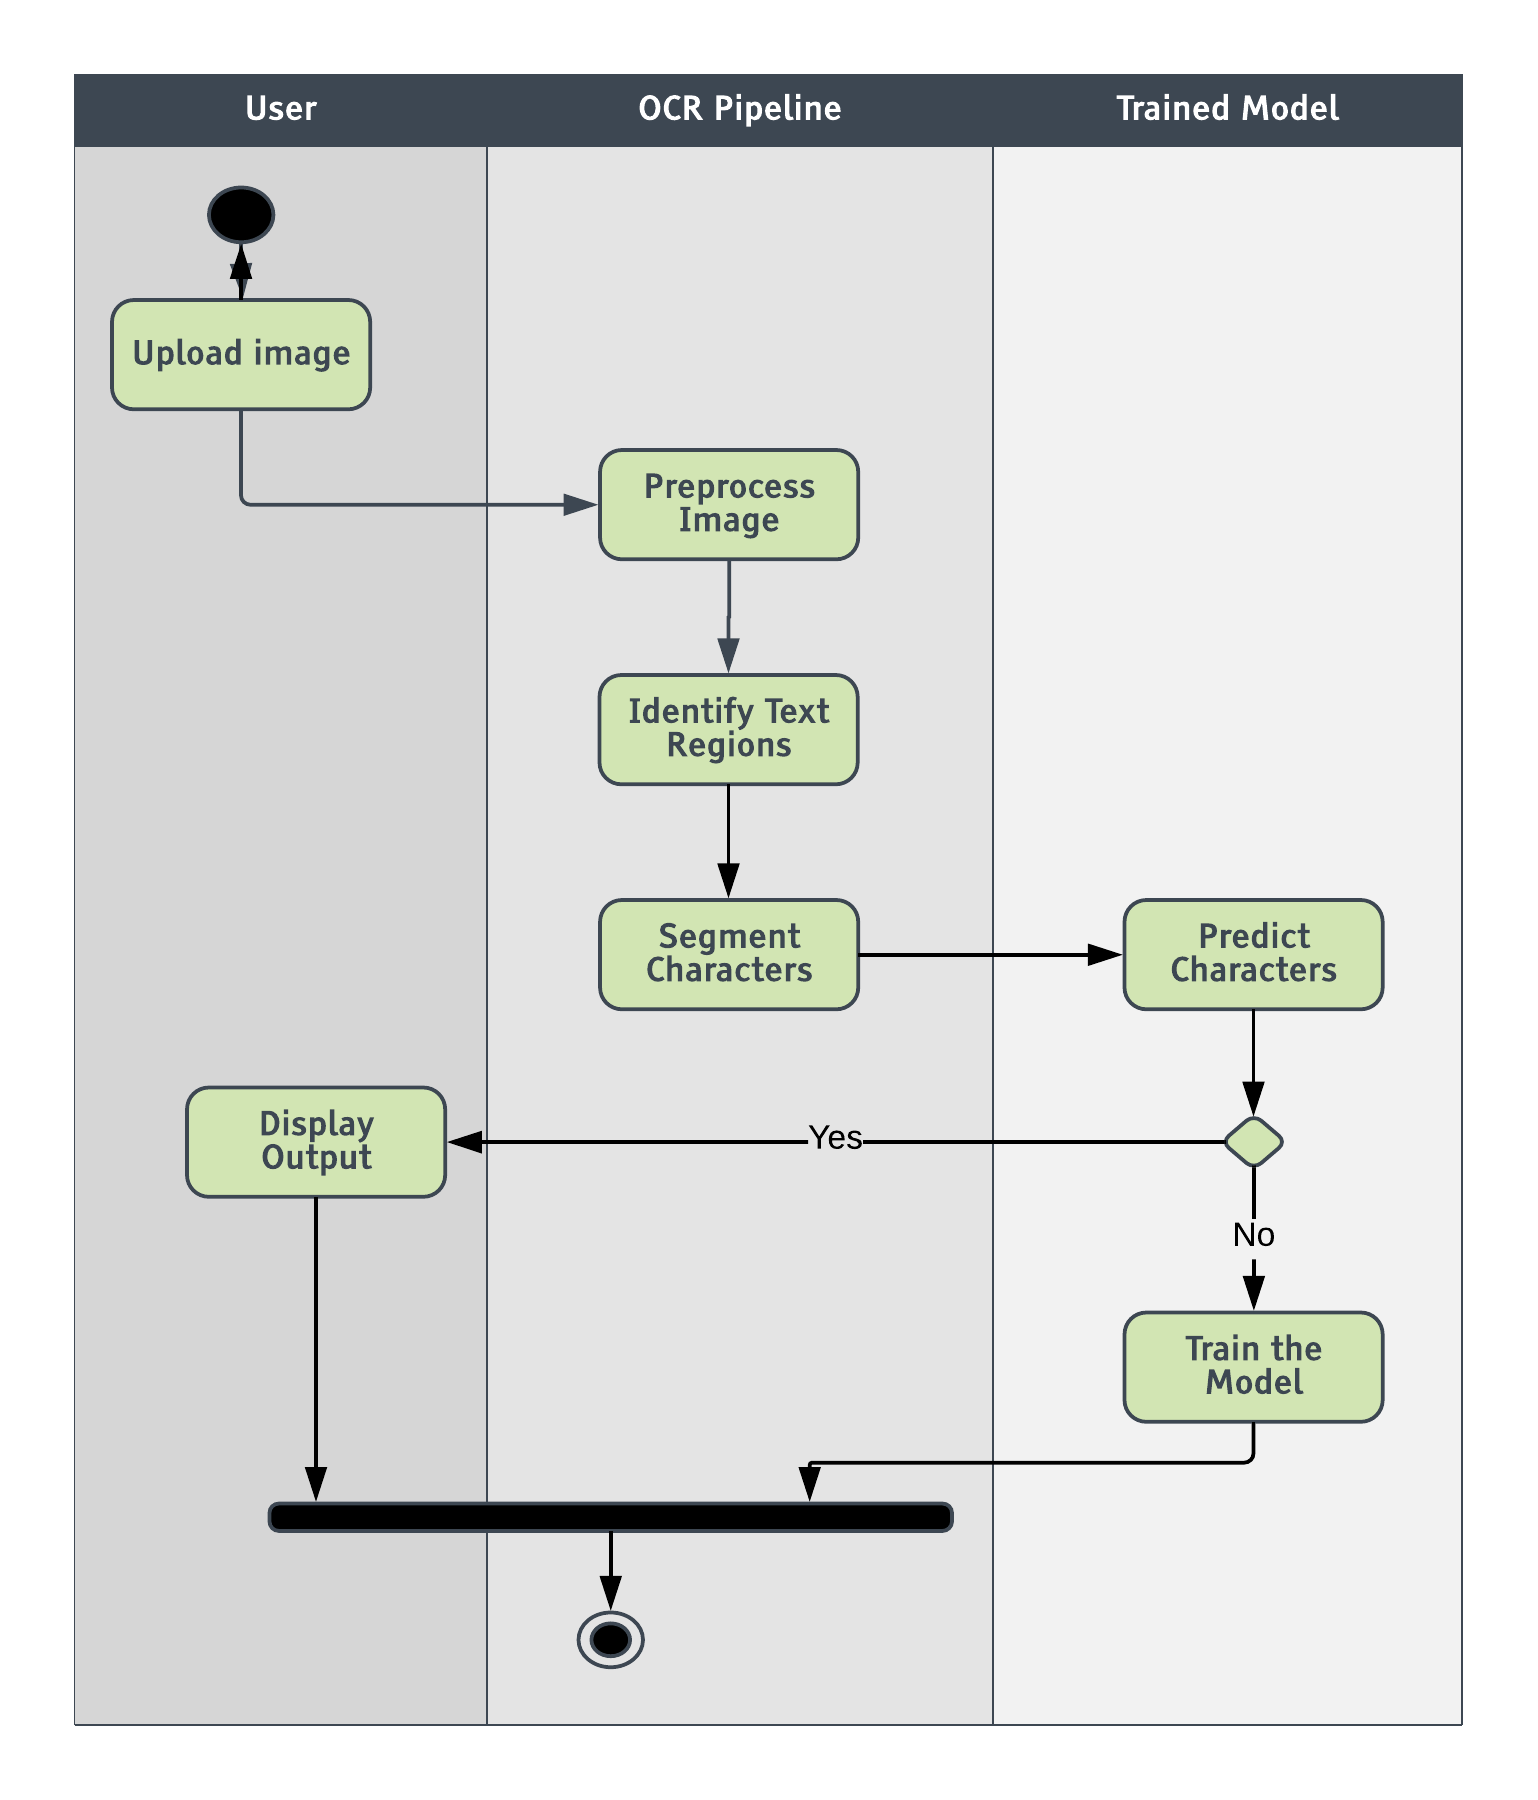
\includegraphics[scale=0.7]{Activity}
\caption{Activity Diagram}
\end{figure}

An activity diagram is essentially a flowchart that shows activities performed by a system. 
The major activities in our system is outlined in the green rounded rectangles. This includes all the major portions of the data flow diagrams as well as the decision making steps carried out to give the output to the user.

\section{Training and recognition}
To do character recognition we used Python Programming Language along with neural network tools like Tensorflow, Keras, etc and some image processing tools like Scipy, OpenCV. The whole process is divided into the following categories:

\begin{itemize}
    \item Training Architecture:
We used Convolutional Neural Network (CNN) as neural network. The CNN used is sequential model which consists of nine layers with four convolutional layers excluding the input and output layers.
    \item Pre-processing of the image for creation of dataset(in CSV file):
First of all, we converted each image of the datasets into grayscale and converted it into numerical two dimensional arrays corresponding to the pixel intensity of each image and saved the arrays in CSV file appending the label of character of each image to each array. The data arrays were arranged randomly for the better training of the datasets.
    \item Training and Testing of the network:
For training, 80\% of the datasets were taken and the remaining were used for cross validation and testing. The datasets were used 10 times i.e for 10 times we trained the CNN with same datasets. So, the whole process of training \& testing took about 15 minutes and the accuracy obtained was about 86\%.   
    \item Recognition:
\begin{figure}[htb]
\centering
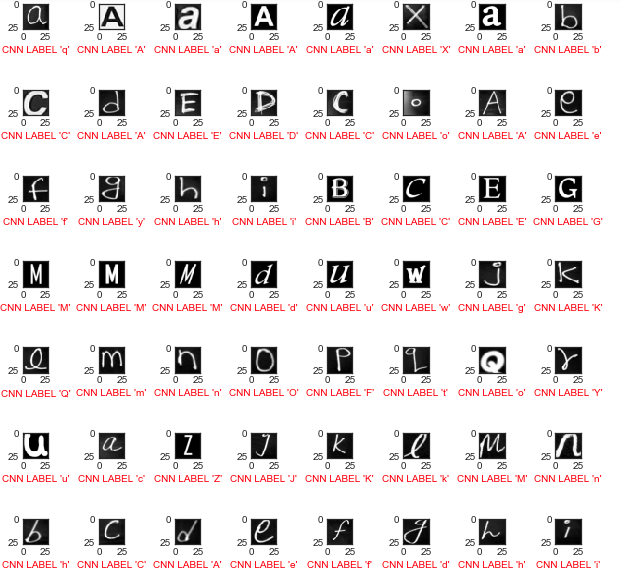
\includegraphics[scale=0.5]{recog}
\caption{Training images for our model}
\end{figure}

Recognition is same as that of testing. The image which is to be recognized is passed into image processor for conversion of it into gray-scaled array of the pixel intensity and passed into predictor function which predicts the label of the image.
\end{itemize}







\chapter{Result}
First we got our hands dirty with MNIST datasets and Neural Network with the help of the book Make Your Own Neural Network \autocite{make_own}. The output from the model trained from this dataset for digits recognition was 97\%.

Then we approached Optical Character Recognition problem with divide and conquer. We first enlisted all the possible algorithms/models. Then we shortlisted the models and bruteforced each model individually and compared the results. Again we re-evaluated our models and tried to optimize our model further by parameter tuning. Then we finally compared the results and decided to use neural networks since it gave best result at reasonable latency.

\section{Output}
When we trained our model with MNIST dataset for digit recognition, it gave accuracy of 97\%. 

We used 74 k datasets for our training model. This dataset contains 74000 sets of data with 62 categories including capital and small letters and 10 digits. Thus trained model was firstly 83\% accurate. Later we improved it to 86\% accuracy with parameter tuning and optimizations.

\section{Comparision}
Comparing the system with other available systems, our system performs decently. Most of the Optical Character Recognition Systems have accuracy in the range of 80-95\%. 

However, we also developed a web front-end for our system which makes the system accessible to the end-users. Most of the other systems are just APIs or command line tools that are not so usable for the end users. In this regard, our systems stands out.

\chapter{Conclusion}

In this project, an OCR system has been developed which employs Maximally Stable Extremal Regions as basic letter candidates. To overcome the sensitivity of MSER with respect to image blur and to detect even very small letters, a modified version of MSER complimented with the Canny edges is used. The detected text are binarized letter patches, which are directly used for text recognition purposes. CNN does not require specific feature to be added as input. It works on the raw pixel of image and extracts features from there based on the number of layers and the number of neurons in each layers. The system worked with an accuracy of around 83\% which makes us confident for using it in recognizing handwritten as well as printed texts.

\section{Limitations}
\begin{enumerate}
\item Accuracy of the system is not satisfactory.
\end{enumerate}

\section{Future Enhancements}
\begin{enumerate}
\item Accuracy of the system can be improved by using a much larger dataset.
\item Second, the CNN architecture can be improved further to include more features.
\item Pre-processing of image can be improved using techniques like stroke width transforms which provides a much greater confidence in identifying text regions in the image.
\item Extension of the system to identify whole words at a time instead of characters
\item Can be extended to other languages, logos, symbols, and even used in vehicle plate recognition.
\end{enumerate}

\printbibliography
\end{document}
